\documentclass[a4paper,12pt]{article}
\usepackage[utf8]{inputenc}
\usepackage[T1]{fontenc}
\usepackage{setspace} % This package is used to control linespacing; With \onehalfspacing for instance
\usepackage[danish]{babel}
\renewcommand{\danishhyphenmins}{22} % bedre orddeling
\usepackage{bm}
\usepackage{fnbreak}
\usepackage{sectsty}
\usepackage{wrapfig}
\usepackage[scriptsize]{caption}
\usepackage[danish,textsize=tiny,backgroundcolor=red,bordercolor=blue]{todonotes}
\usepackage[isbn,issn]{dk-bib}
\interfootnotelinepenalty=10000
\usepackage{graphicx}
\usepackage{usecases}
\usepackage{pdfpages}

\addto\captionsdanish{
\renewcommand\abstractname{Abstract}
}
%-----------------------------------------------------
\newcommand{\doctitle}{Eksaminations projekt}
\newcommand{\docsubject}{Software Engineering 1(02161)}
\newcommand{\docauthor}{Christian Kiær s123812, Carsten Rosenkilde Nielsen s123062 og Jonathan Becktor s123094}
\newcommand{\docdate}{\today}
\newcommand{\docplace}{Danmarks Tekniske Universitet}
\newcommand{\HRule}{\rule{\linewidth}{0.5mm}}
%\newcommand{\docsubtitle}{Undertitle}
%-----------------------------------------------------

%-----------Scientific and mathematical packages begin-----------
% Math package
	\usepackage{amsmath}

% Vector symbols and functions (for example \vv)
	\usepackage{esvect}

% Mathematical symbols
	\usepackage{amssymb}
\DeclareMathOperator{\p}{\cdot}
\DeclareMathOperator{\N}{\mathbb{N}}
\DeclareMathOperator{\Z}{\mathbb{Z}}
\DeclareMathOperator{\C}{\mathbb{C}}
\DeclareMathOperator{\R}{\mathbb{R}}
\newcommand{\nn}{\nonumber}
% SI Units
	%\usepackage[output-decimal-marker={,}]{siunitx}		%http://mirrors.dotsrc.org/ctan/macros/latex/begincontrib/siunitx/siunitx.pdf
	%\sisetup{unitsep= \cdot }

% For Chemistry
	%\usepackage{chemscheme}		% http://ctan.org/pkg/chemscheme
	%\usepackage{chemsym}		% http://ctan.org/pkg/chemsym
	%\usepackage{mhchem}			% http://mirrors.dotsrc.org/ctan/macros/latex/contrib/chemstyle/chemstyle.pdf
	%\DeclareSIUnit\Molar{\textsc{m}}
%-----------Scientific and mathematical packages end--------------

% Non-default fonts - has to come _after_ some of the mathematical packages
\usepackage{pxfonts}

% Page margins
\usepackage[left=2.0cm, right=1.5cm]{geometry}

% Hyperref
\usepackage[colorlinks=true,linkcolor=black,citecolor=black,urlcolor=black]{hyperref}
%\usepackage[hidelinks]{hyperref}  
\hypersetup{pdftitle={\doctitle}} 
\hypersetup{pdfsubject={\docsubject}}
\hypersetup{pdfauthor={\docauthor}}

% Setspace
\usepackage{setspace}
\onehalfspacing
%\numberwithin{equation}{section}
% Alter some LaTeX defaults for better treatment of figures:
    % See p.105 of "TeX Unbound" for suggested values.
    % See pp. 199-200 of Lamport's "LaTeX" book for details.
    %   General parameters, for ALL pages:
    \renewcommand{\topfraction}{0.9}	% max fraction of floats at top
    \renewcommand{\bottomfraction}{0.8}	% max fraction of floats at bottom
    %   Parameters for TEXT pages (not float pages):
    \setcounter{topnumber}{2}
    \setcounter{bottomnumber}{2}
    \setcounter{totalnumber}{4}     % 2 may work better
    \setcounter{dbltopnumber}{2}    % for 2-column pages
    \renewcommand{\dbltopfraction}{0.9}	% fit big float above 2-col. text
    \renewcommand{\textfraction}{0.07}	% allow minimal text w. figs
    %   Parameters for FLOAT pages (not text pages):
    \renewcommand{\floatpagefraction}{0.7}	% require fuller float pages
	% N.B.: floatpagefraction MUST be less than topfraction !!
    \renewcommand{\dblfloatpagefraction}{0.7}	% require fuller float pages

	% remember to use [htp] or [htpb] for placement

% Title
\title{
\HRule \\
\textsc{\doctitle} \\
	 \small{\textsl{\docsubtitle}}
\HRule
}
\author{\docauthor\\\small{\docplace}}
\date{\docdate}

% Fancyheader : http://mirrors.dotsrc.org/ctan/macros/latex/contrib/fancyhdr/fancyhdr.pdf
\usepackage{fancyhdr}
\pagestyle{fancy}
\fancyhf{}
%\fancyhead[RO]{\docauthor \hfill \doctitle \hfill\thepage}
\fancyhead[RO]{\doctitle \hfill Gruppe 01  \hfill \thepage /\ref{TotPages}}
% Get rid of annoying error messages
\setlength{\headheight}{14.5pt}
\usepackage{totpages}
\usepackage{sectsty}
\allsectionsfont{\scshape}
\begin{document}
\begin{titlepage}
\begin{center}
\textsc{\LARGE Danmarks Tekniske Universitet}\\[1.5cm]
\textsc{\large Eksaminations Projekt}\\[0.5cm]
\HRule \\[0.4cm]
{ \huge \bfseries Project Planner}\\[0.1cm]
\HRule \\[1.5cm]
\end{center}
\begin{flushleft} \large
\emph{Gruppemedlemmer:}\\
Carsten Michael Rosenkilde \textsc{Nielsen} s123062\\
Christian Mathias Rohde \textsc{Kiær} s123812\\
Jonathan Binner \textsc{Becktor} s123094\\
\end{flushleft}
\vfill 
\begin{center}
{\large \today}
\end{center}
\end{titlepage}
\section*{Indledning}
Til opgave har vi fået stillet, at designe en planlægningsapplikation. Denne applikation skal skabes for et softwarehus, der mangler et system til at planlægge deres projekter. Projekter skal kunne oprettes efter de informationer, der haves på oprettelses tidspunktet. Dette skal kunne inkludere navn, start/sluttidspunkt og projektleder. Alle disse oplysninger skal også kunne tilføjes eller ændres senere hen. Projekter skal kunne tildeles aktiviteter, som tilføjes med et navn, en beskrivelse,en start/slut dato, antal  allokerede timer og det aktuelle timeforbrug. Udviklere skal kunne tildeles aktiviteter, og derfra registrere deres timeforbrug på den pågældende aktivitet. Til løsning af problemerne, har vi opstillet 6 Use Cases som vi vil implementere testdrevent.  \\
Følgende Use Cases har vi valgt at kigge på: 
\begin{itemize}
\item Create projects
\item Manage projects
\item Define Activities
\item Manage developers
\item Hours worked on project
\item Seek Assistance
\end{itemize}
Vi har implementeret alle Use Cases test drevent, og det er gjort i forbindelse og uden konflikt med opgavebeskrivelsen.
\newpage
\tableofcontents
\newpage
\section{Kravspecifikation}
\subsection{Væsentlige begreber}
Under udviklingen har vi oprettet føglende liste af vigtige begreber:
\begin{itemize}
\item User: skal forstås som brugeren eller udviklerne
\item Project: Projektet eller opgaven der er stillet softwarehuset. Projekter kan være tildelt navn og projektleder. Projekter kan også have deadlines.
\item Activity: Aktiviteter er opgaverne tilknyttet projekterne. Udviklere skal kunne være tilknyttet en aktivitet og registrere deres arbejdstid. Aktiviteter kan være tildelt navn, beskrivelse og deadlines.
\item Projectleader: Projektlederen er den ansvarlige udvikler for et projekt.
\item Available developers: Det skal være muligt for både projektleder og udviklere, at finde udviklere der er tilgængelige til enten hjælp eller tildeling af aktivitet.
\item Administrator: Superbrugeren af systemet. Administrator skal kunne registrere brugere og oprette projekter.
\item Work: Udviklerne skal have en let måde at registrere det antal timer de har arbejdet på et givent projekt. Gennem work kan de nemt registrere dette, samt hvilken aktivitet de var tilknyttet.
\end{itemize}
Disse begreber er væsentlige for forståelsen af udviklingen af programmet, og de tanker der er gjort bag. Dette er de begreber, vi har defineret ud fra opgavebeskrivelsen og de use cases der er blevet opstillet.
\subsection{Use cases}
Alle vores Use cases ligger som bilag. Se bilaget for at finde de pågælende use cases.
\subsubsection*{Use case 1}
Vores første use case, beskriver hvordan projekter skal oprettes. Se bilag Use case 1.
\subsubsection*{Use case 2}
Vores anden use case, beskæftiger sig med modifikationen af projekter. Se bilag Use case 2.
\subsubsection*{Use case 3}
Se bilag Use case 3.
\subsubsection*{Use case 4}
Se bilag Use case 4.
\subsubsection*{Use case 5}
Se bilag Use case 5.
\subsubsection*{Use case 6}
Se bilag Use case 6.
\newpage
\section{Programdesign}
\subsection{Klasser}
\begin{figure}[htp]
\centering
\includegraphics[scale=0.25]{classdiagram.jpg}
\caption{Klassediagram}
\label{fig: Klassediagram}
\end{figure}
Ovenfor er vores klassediagram opstillet. Vi har valgt kun at vise de public metoder, for alle vores klasser. Derudover viser diagrammerne hvilke funktioner, der kan hente oplysninger fra hvad.
\newpage
\subsection{Sekvensdiagrammer}
\begin{figure}[htp]
\centering
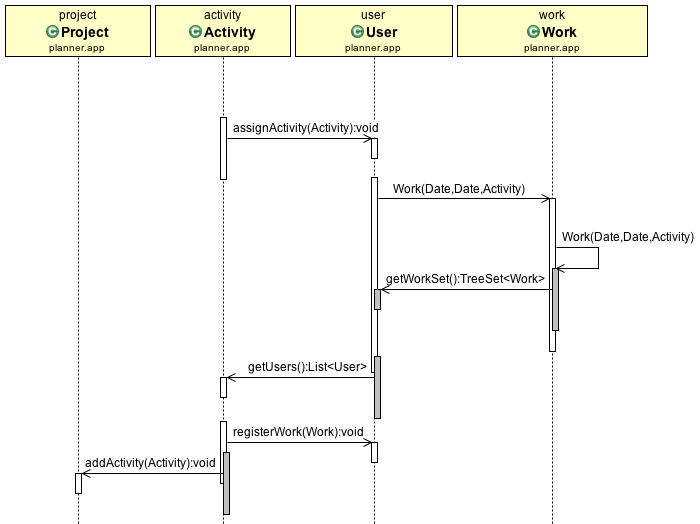
\includegraphics[scale=0.5]{seq1.png}
\caption{Workhours}
\end{figure}
asdasdasd
asdasdasd\\asdads\\asdasd

\begin{figure}[htp]
\centering
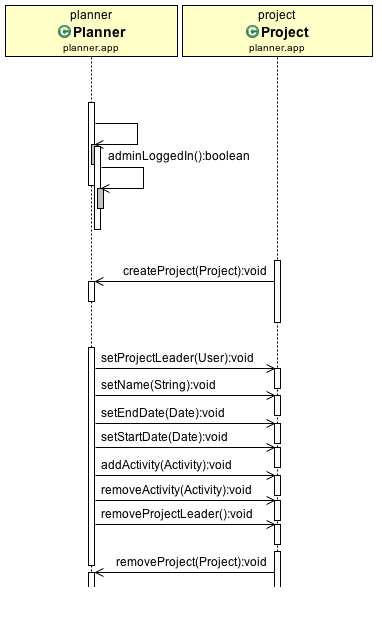
\includegraphics[scale=0.5]{seq2.png}
\caption{Project creation and modification}
\end{figure}
asdasdasd
asdasdasd\\asdads\\asdasd
\newpage
\begin{figure}[htp]
\centering
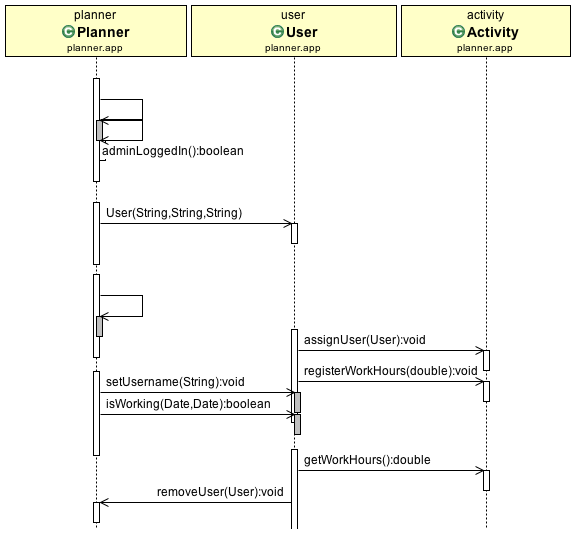
\includegraphics[scale=0.5]{seq3.png}
\caption{User creation and modification}
\end{figure}
asdasdasd
asdasdasd\\asdads\\asdasd\\
asdasdasd
asdasdasd\\asdads\\asdasdasdasdasd
asdasdasd\\asdads\\asdasdasdasdasd
asdasdasd\\asdads\\asdasdasdasdasd
asdasdasd\\asdads\\asdasdasdasdasd
asdasdasd\\asdads\\asdasdasdasdasd
asdasdasd\\asdads\\asdasd
\newpage
\subsection{Diskussion}
Vi som gruppe diskuterede vi hvad der skulle lægges fokus på. Til at starte med var vi enige om at der skulle være GUI, persistency og god funktionalitet. Dog da vi var et godt stykke inde valgte vi at fokusere på programmets funktionalitet og de tilhørende tests for at få så god "code coverage" som muligt. Da alle vores use cases kun beskæftiger sig med funktionalitet af programmet, kunne vi derfor opnå at færdiggøre dem alle. Dette medfører også, at vores use cases har tests for de fleste scenarioer.\\
Oplægget til opgaven skaber en del uklarheder rundt omkring, der dog let kan ændres på. Specielt de forskellige brugers rettigheder i programmet, var vi i tvivl om. Derfor er programmet meget åbent, og kun nogle få metoder kræver brugerrettigheder. 
\section{Systematiske test}
Alle vores tests er i bund og grund lavet for at kunne få så høj "code coverage" som muligt. Med dette som bagrund har vi lavet tests til mere eller mindre alt i programmet. Vi har taget brug af EclEmma for at finde hvor vi manglede test og hvad der ikke var covered. Nogle af de oftest funde test er tests for getters \& setters hvilket var forholdsvist let at få testet man laver en værdi som sættes i en setter hvorefter vi bruger assertEquals for at se om den værdi vi har sat i setteren er den samme vi får fra getteren når vi spørger efter den. En anden test der ofte skulle testes var hvis fx. en setter ikke kunne være null og hvis den var skulle kaste en fejl. Her bruger vi try/catch i testsne for at fange de fejl som programmet giver os og sammenligner dem med de ønskede fejlmeddelelser.

\subsection*{Usecase 1. Create Project}
Vi tester om admin er logget ind. Derefter kan administratoren lave projekter. Hvis administratoren laver et projekt uden navn vil programmet tildele den et. Dette testes ved at lave et program uden navn og derefter teste ved getName metoden om navnet er blevet til "default name". Denne slags test bliver brugt flere gange i denne usecase hvis der ikke skrives start dato bliver den af default sat til dags dato. dette tjækkes på samme måde. Hvis projektet bliver lavet med end date før start date kaster programmet en fejl. Denne fanger vi med en try/catch som tjekker om fejlen og fejlmeddelelsen er det samme.

\subsection*{Usecase 2. Manage Project}
Vi tester her om Projekt leader kan ændre i projects, vi tester om der kan ændres i navn, startdato, slutdato og hvordan programet håndterer det. Der testes også om projektleder kan skiftes ud. Derudover tester vi om der kan ændres i activities og hvordan det håndteres hvis man skal fjerne en activity.

\subsection*{Usecase 3. Define activities}
Først testes det om en user kan lave "activities", derefter testes det om users kan skifte navn, beskrivelse og "allocated workhours". Derefter kan vi teste hvad der sker hvis man undlader et navn på activity, hvad der sker hvis man giver negative "workhours" og hvordan vil programmet håndtere at man giver den eksempelvis en startdato uden slut dato eller omvendt. Der skal også testes hvad der sker hvis slut dato er før start dato.

\subsection*{Usecase 4. Manage Developers}
Her tester vi først om admin kan lave "developer", hvorefter der testes om der kan ændres username, email og password. Der testes for hvad der sker hvis man ændrer enten username, email eller pasword til null. Derudover testes der også for identiske users.

\subsection*{Usecase 5.Hours worked on project}
Først tester vi om User kan finde "activities", derefter tester vi at user kan skrive antal timer brugt på "activity" hvorefter vi tester om de blicer registreret i work. Vi tester også om en Developer kan sætte sig selv som working. Vi bliver også nød til at teste hvis der ikke bliver indsat en activity. Der testes for at hvis user indsætter mere "allocated hours" end hvad der er tid i projektet og der testes for minus tid.
\subsection*{Usecase 6.}
Vi laver en test for at en user kan skulle kunne hente en liste af developers. Derudover tester vi om user kan se de andre developers "Work" for at se om de arbejder på en activity.

\section{Konklusion}
Vi har fået skabt et program, der lever op til de kravspecifikationer vi har fået stillet. Programmet er gennemtestet med mange scenarioer, og derfor har vi prøvet at sikre en høj kvalitet. Der er plads til udvidelse, hvis dette skulle være at ønske. Af egenskaber vi ikke har nået, som dog ikke er en del af kravspecifikationerne, kan nævnes et persistency layer og et UI. Dette er selvfølgelig påkrævet for et fuldt funktionelt program. Vi har dog opnået at få skabt det grundlæggende, for en planlægningsapplikation.\\ 
Projektet har forløbet fint. Dog har der grundet andre kurser været funktioner vi har måtte udelade. Derfor har vores fokus været på de grundlæggende funktioner, og ting funktioner vi havde tiltænkt, som GUI og persistency, blev udeladt. Dette er dog noget vi i sidste ende har været glade for, da det har givet os bedre tid til at løse vores use cases. I forhold til vores oprindelige projektplan, kom vi forsent igang allerede fra uge 1. Dette medførte de fornævnte fravalg. Dette var dog noget vi blev enige om forholdsvist hurtigt. Ellers vil vi mene at vi har forsøgt at følge planen, og har prøvet at have så få overskridelser af tiden som muligt.\\
Alt i alt har dette givet os en mulighed, for at prøve at arbejde mod en deadline. Vi har fået indblik i hvilke valg der skal tages, og har indset at ikke alle de ideer man har gjort sig nødvændigvis kan nås.
\newpage
\section{Bilag}
\subsection{Use case 1}
\begin{usecase}

\addtitle{Use Case 1}{Create Project} 

%Scope: the system under design
\addfield{Scope:}{System-wide}	
%Primary Actor: Calls on the system to deliver its services.
\addfield{Primary Actor:}{Administrator}

%Stakeholders and Interests: Who cares about this use case and what do they want?
\additemizedfield{Stakeholders and Interests:}{
	\item Administrator: Needs to be able to create and modify projects
	\item Project Leader: Needs to modify projects and add activities to projects
	\item Developer: Needs to be able to see projects
	
}
\addfield{Description:}{Makes it possible to create a project}
%Main Success Scenario: A typical, unconditional happy path scenario of success.
\addscenario{Main Scenario:}{
	\item Gives the administrator the possibility to create projects
	\item The administrator will be able to create with a given name and projectleader.
	\item The administrator can assign a start and end date to the project
}

%Extensions: Alternate scenarios of success or failure.
\addscenario{Alternative Scenarios:}{
	\item[1.a] Invalid login data:
		\begin{enumerate}
		\item[1.] System shows failure message
		\item[2.] System returns to step 1
		\end{enumerate}
	\item[2.a] No projectleader assigned:
		\begin{enumerate}
		\item[1.] If projectleader is not assigned, it will create the proejct with no projectleader.
		\item[2.] Administrator will be able to set the projectleader by modifying the project
		\end{enumerate}
	\item[2.b] No projectname assigned:
		\begin{enumerate}
		\item[1.] If projectname is not assigned, a default name will be assigned
		\item[2.] Administrator or proejctleader will be able to change the name, by modifying the project.
		\end{enumerate}
	\item[3.a]  If start date not assigned:
		\begin{enumerate}
		\item[1.] If start are not assigned the project will be created with the current date as start date.
		\end{enumerate}
	\item[3.b] If end date not assigned:
		\begin{enumerate}
		\item[1.] If end date is not assigned, the project will be created with no value as end date.
		\end{enumerate}
	\item[3.c] End date is before start date
		\begin{enumerate}
		\item[1] The system automaticly changes the end date to be after the start date.
		\end{enumerate}
}
\end{usecase}
\newpage
\subsection{Use case 2}
\begin{usecase}

\addtitle{Use Case 2}{Manage Project} 

%Scope: the system under design
\addfield{Scope:}{System-wide}

%Primary Actor: Calls on the system to deliver its services.
\addfield{Primary Actor:}{Project Leader}

%Stakeholders and Interests: Who cares about this use case and what do they want?
\additemizedfield{Administrator, Project Leader:}{
	\item Administrator: Assign project leader.
	\item Project Leader: Assign activities to project and manage them.
}

%Preconditions: What must be true on start and worth telling the reader?
\addfield{Description:}{Makes it possible to assign a project leader, change project leader and assign and manage activities to project}
%when multiple
%\additemizedfield{Preconditions:}{} 

%Main Success Scenario: A typical, unconditional happy path scenario of success.
\addscenario{Main Success Scenario:}{
	\item Admin assigns project leader.
	\item Project leader assigns activities to project.
	\item Project now managed.
}

%Extensions: Alternate scenarios of success or failure.
\addscenario{Alternative Scenarioes:}{
	\item[1.a] Admin assigns wrong project leader:
		\begin{enumerate}
		\item[1.] Admin changes project leader.
		\item[2.] Project Leader continues on step 2.
		\end{enumerate}
	\item[1.b] Admin assigns invalid project leader:
		\begin{enumerate}
		\item[1.] System shows failure message
		\item[2.] Admin assigns correct project leader
		\end{enumerate}
		
	\item[2.a] Wrong activity data:
		\begin{enumerate}
		\item[1.] Project leader corrects activity data
		\item[2.] Project leader continues with step 3
		\end{enumerate}
	\item[2.b] Invalid activity data:
		\begin{enumerate}
		\item[1.] System shows failure message
		\item[2.] Project leader returns to step 2 and corrects the errors
		\end{enumerate}
	\item[2.c] Wrong activity:
		\begin{enumerate}
		\item[1.] Project leader removes activity
		\item[2.] Project leader returns to step 2
		\end{enumerate}	
}
\end{usecase}
\newpage
\subsection{Use case 3}
\begin{usecase}

\addtitle{Use Case 3}{Define activities} 

%Scope: the system under design
\addfield{Scope:}{System-wide}	
%Primary Actor: Calls on the system to deliver its services.
\addfield{Primary Actor:}{Project leader and Developer}

%Stakeholders and Interests: Who cares about this use case and what do they want?
\additemizedfield{Stakeholders and Interests:}{
	\item Project Leader: Needs add activities to projects and modify them.
	\item Developer: Needs add activities to projects and modify them. Also needs to register hours worked on given activity.
	
}
\addfield{Description:}{Makes it possible to create an activity connected to a project, add developers to the activity and assign workhours to the activity}
%Main Success Scenario: A typical, unconditional happy path scenario of success.
\addscenario{Main Scenario:}{
	\item Lets the users create activities.
	\item The users can create activities, defined by name, description and allocated workhours.
	\item Lets the user connect developers to an activity.
	\item Lets the users define the expected start and end dates of the activity. It's possible to assign an endDate without startDate and vice versa.
	\item Lets the developers define the actual hours of work put into the activity. It's possible to set the final workhours and add work hours while working.
}

%Extensions: Alternate scenarios of success or failure.
\addscenario{Alternative Scenarios:}{
	\item[2.a] No name assigned:
		\begin{enumerate}
		\item[1.] The activity will be assigned a default name.
		\item[2.] The activitys name can be modified at a later time
		\end{enumerate}
	\item[2.b] Description not assigned:
		\begin{enumerate}
		\item[1.] The activity will have no description.
		\item[2.] The description of the activity can be set at a later time.
		\end{enumerate}
	\item[3.a] Adding same user twice
		\begin{enumerate}
		\item[1.] System throws an error
		\item[2.] System returns to 3.
		\end{enumerate}
	\item[4.a]  If start date not assigned:
		\begin{enumerate}
		\item[1.] If start date is not assigned the activity will have no start date.
		\item[2.] The start date can be modified later.
		\end{enumerate}
	\item[4.b] If end date not assigned:
		\begin{enumerate}
		\item[1.] If end date is not assigned, the activity will have no end date.
		\item[2.] The end date can be modified later.
		\end{enumerate}
	\item[4.c] End date is before start date
		\begin{enumerate}
		\item[1.] The system will show an error.
		\item[2.] The system will go back to 4.
		\end{enumerate}
	\item[5.a] Define negative hours of work
		\begin{enumerate}
		\item[1.] System returns an error
		\item[2.] System returns user to 5.
		\end{enumerate}
}
\end{usecase}
\newpage
\subsection{Use case 4}
\begin{usecase}

\addtitle{Use Case 4}{Manage Developers} 

%Scope: the system under design
\addfield{Scope:}{System-wide}

%Primary Actor: Calls on the system to deliver its services.
\addfield{Primary Actor:}{Admin}

%Stakeholders and Interests: Who cares about this use case and what do they want?
\additemizedfield{\textsl{Administrator}:}{
	\item Administrator: Create Developers and manage them.
}

%Preconditions: What must be true on start and worth telling the reader?
\addfield{Description:}{Makes it so admin can manage all information in developers, add and remove new developers.}
%when multiple
%\additemizedfield{Preconditions:}{} 

%Main Success Scenario: A typical, unconditional happy path scenario of success.
\addscenario{Main Success Scenario:}{
	\item Admin creates developer
	\item Admin changes developer username
	\item Admin changes developer email
	\item Admin changes developer password
	\item Developer now managed
}

%Extensions: Alternate scenarios of success or failure.
\addscenario{Alternative Scenarioes:}{
	\item[1.a]Admin creates wrong developer
		\begin{enumerate}
		\item[1.] Admin removes developer
		\item[3.] Admin returns to step 1.
		\end{enumerate}
	\item[2.a] Admin sets null username:
		\begin{enumerate}
		\item[1.] System shows failure message
		\item[2.] Admin changes developer username properly
		\item[3.] Admin continues with step 2
		\end{enumerate}
	\item[3.a] Admin sets null email:
		\begin{enumerate}
		\item[1.] System shows failure message
		\item[2.] Admin changes developer email properly
		\item[3.] Admin continues with step 3
		\end{enumerate}
	\item[4.a] Admin sets null password:
		\begin{enumerate}
		\item[1.] System shows failure message
		\item[2.] Admin changes developer password properly
		\item[3.] Admin continues with step 4
		\end{enumerate}	
}

\end{usecase}
\newpage
\subsection{Use case 5}
\begin{usecase}

\addtitle{Use Case 5}{Hours worked on project} 

%Scope: the system under design
\addfield{Scope:}{System-wide}	
%Primary Actor: Calls on the system to deliver its services.
\addfield{Primary Actor:}{Developer}

%Stakeholders and Interests: Who cares about this use case and what do they want?
\additemizedfield{Stakeholders and Interests:}{
	\item Developer: The developers needs to be able to set themselves as working, and register the hours they are working 
	
}
\addfield{Description:}{Makes it possible for a developer to get set himself as working, and register the ammount of hours he is working}
%Main Success Scenario: A typical, unconditional happy path scenario of success.
\addscenario{Main Scenario:}{
	\item User finds activity
	\item User enters hours spent on activity
	\item Activity registers hours Developer has spent.
}

%Extensions: Alternate scenarios of success or failure.
\addscenario{Alternative Scenarios:}{

	\item[1.a] User set to work:
		\begin{enumerate}
		\item[1.] Sets himself to working
		\end{enumerate}
		
	\item[1.b] Non existent activity:
		\begin{enumerate}
		\item[1.] System casts errormessage.
		\item[2.] Returns to step 1.
		\end{enumerate}
		
	\item[1.c] null activity:
		\begin{enumerate}
		\item[1.] System casts errormessage.
		\item[2.] Returns to step 1.
		\end{enumerate}
		
	\item[2.a] allocated hours more than actual time on project:
		\begin{enumerate}
		\item[1.] System casts errormessage.
		\item[2.] returns to step 2.
		\end{enumerate}
	
	\item[2.b] negative work hours:
		\begin{enumerate}
		\item[1.] System casts errormessage.
		\item[2.] returns to step 2.
		\end{enumerate}
		
	\item[3.a] allocated hours more than actual time on project:
		\begin{enumerate}
		\item[1.] System casts errormessage.
		\item[2.] returns to step 2.
		\end{enumerate}
			
}
\end{usecase}
\newpage
\subsection{Use case 6}
\begin{usecase}

\addtitle{Use Case 6}{Seek assistence} 

%Scope: the system under design
\addfield{Scope:}{System-wide}	
%Primary Actor: Calls on the system to deliver its services.
\addfield{Primary Actor:}{Developer}

%Stakeholders and Interests: Who cares about this use case and what do they want?
\additemizedfield{Stakeholders and Interests:}{
	\item Developer: Needs to be able to see which developers are available, at the given time. 
	
}
\addfield{Description:}{Makes it possible for developers to see which developers is not currently working on an activity}
%Main Success Scenario: A typical, unconditional happy path scenario of success.
\addscenario{Main Scenario:}{
	\item Lets the user get a list of developers.
	\item The user can see which developers is not working on an activity.
}

%Extensions: Alternate scenarios of success or failure.
\addscenario{Alternative Scenarios:}{
	\item[2.a] Requires work to not overlap:
		\begin{enumerate}
		\item[1.] If work overlaps, system cast error.
		\item[2.] Returns to 1.
		\end{enumerate}
}
\end{usecase}
\newpage
\subsection{Original tidsplan}
\begin{figure}[h]
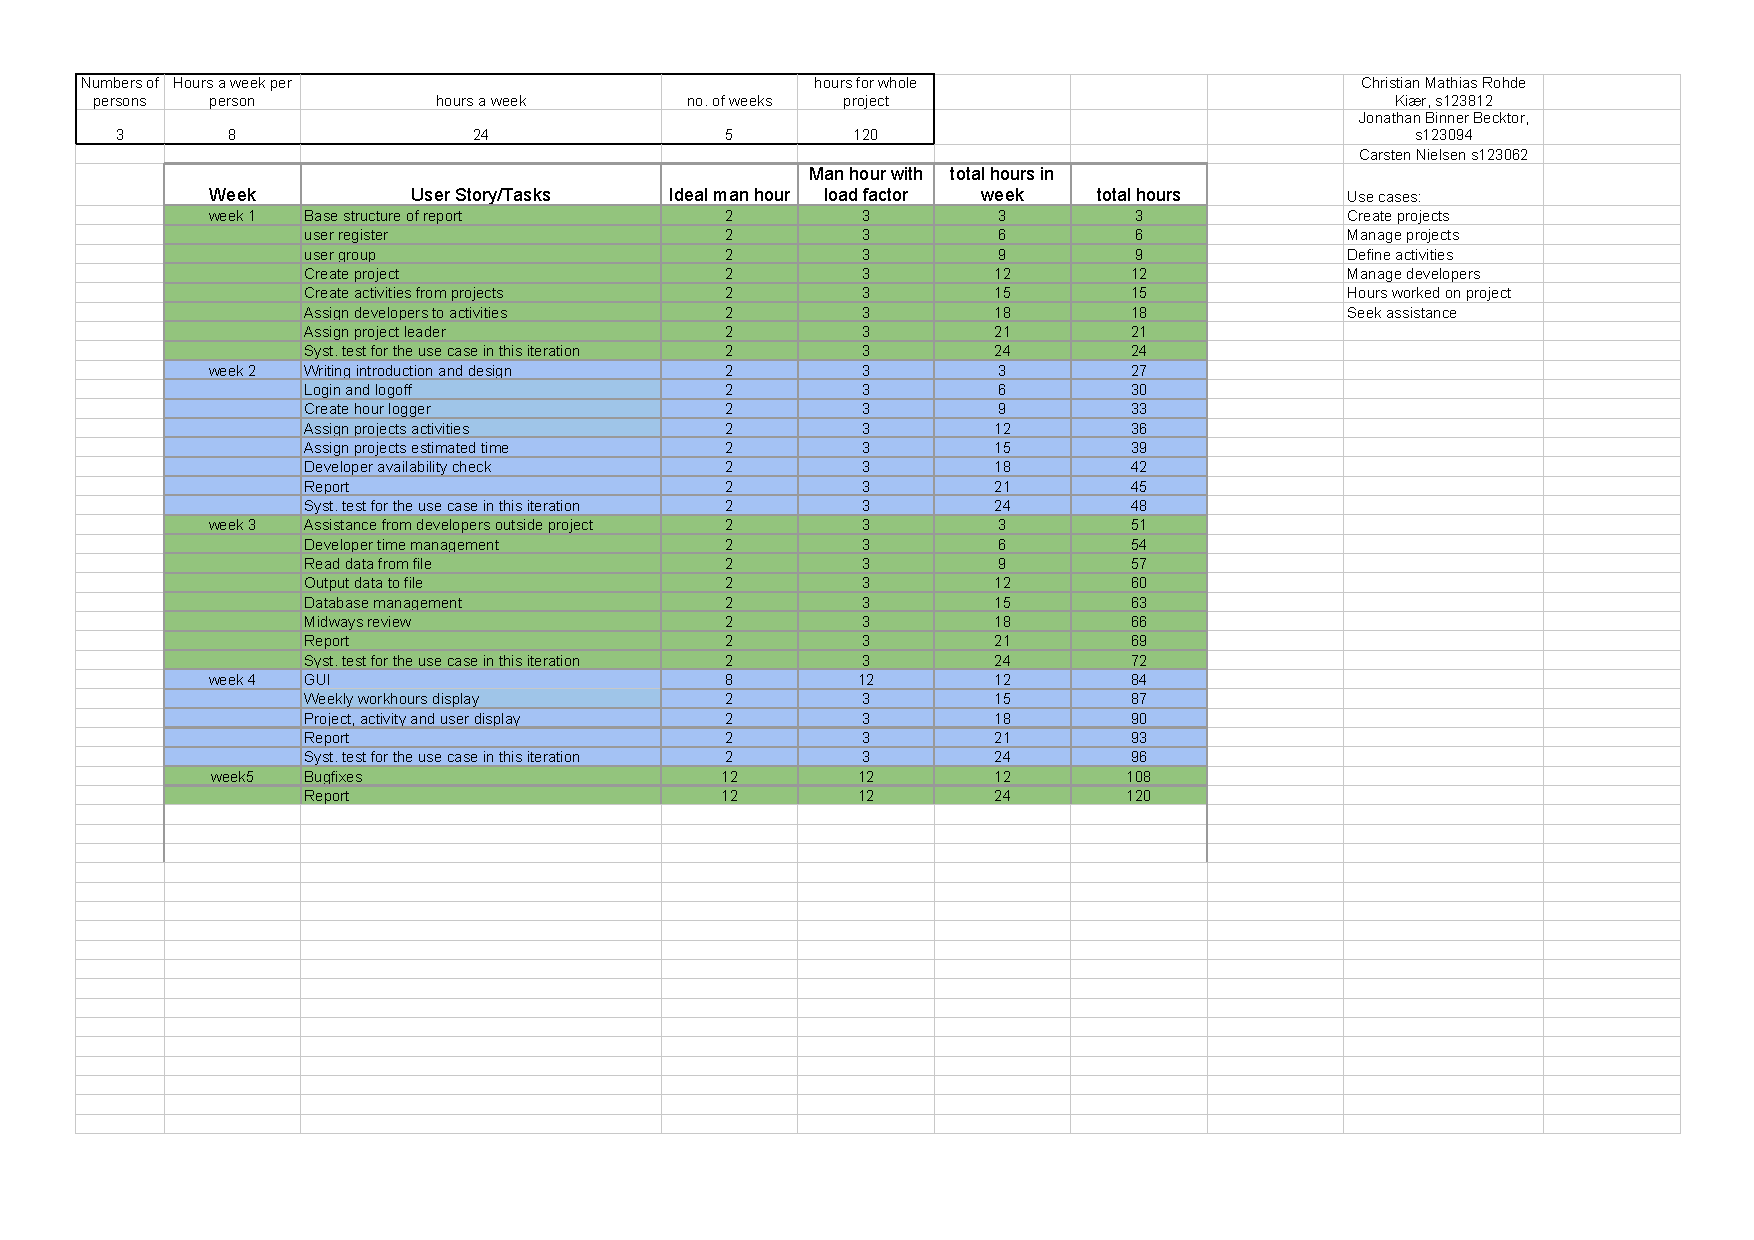
\includepdf[pages={1}]{SOFTWARE.pdf}
\caption{Oprindeligt planlægningsark}
\end{figure}
\end{document}